\section{Introduction}\label{sec:collab:Introduction}

\label{sec:collab}
When collaborating with other groups about the different design aspects we needed to have the different design requirements from the requirements group.
When we got them, we arranged a meeting and discussed the different requirements and created design conventions for each user story.
In this project we worked together with the iOS and Life-stories groups.
The first meeting concentrated on which common settings we should make and where they should be placed. In the launcher or in the application itself. 
Another thing we discussed was the common requirements for iOS, sequence, and Life-stories. 

Here are the following things we agreed upon.
\begin{itemize}
\item Extending the database to have the ability to save a sequence to a database
\item Marking a pictogram as "done" when the user has done the activity for that pictogram.
\end{itemize}

The following list are only between sequence and lifestories. 
\begin{itemize}
\item Share our codes because most of sequences functionality can be used in Life-stories
\item Implementing landscape and portrait-mode. This should be able to lock, so the tablet does not accidentally switch in between them. Therefore there should be a button to switch in between them.
\item The settings should be saved for each child.
\end{itemize}

Because of Life-stories wanted to have much of sequences' functionality we decided to make another application which has the purpose of showing a sequence, and maybe highlighting the pictogram as "done".

In the next meeting we showed our applications and we made an ER (entity relationship) diagram to show how storing a sequence in a database would be handled.
We agreed upon that the database design should look like \ref{fig:Sequence-tables}:
\begin{figure}
\centering
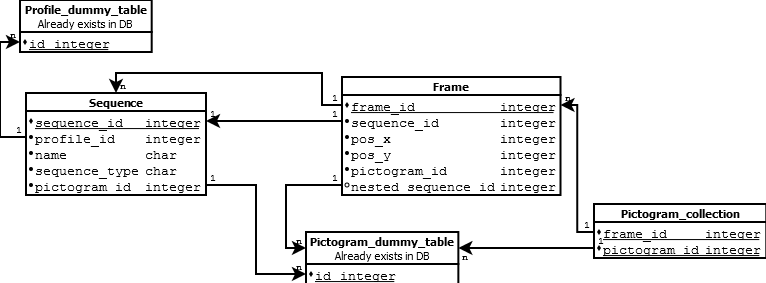
\includegraphics[width=0.7\linewidth]{Pics/Sprint2/Sequence-tables}
\caption[An ER diagram that should be included into the overall database]{}
\caption{}
\label{fig:Sequence-tables}
\end{figure}
We agreed that the Life-stories group will collaborate with the Database group on extending and adjusting the database.
We should work upon making the new application which will be called "Sequence-Viewer". This application will be used by Life-stories, Sequence, and Parrot. Parrot is the application which will read the sequences. \note{This is also the name of the "Picto-oplæser"}